\documentclass[preprint,12pt,authoryear]{elsarticle}
\usepackage[T1]{fontenc}
\usepackage{amsmath,amssymb}
\usepackage{graphicx}
\usepackage{booktabs}
\usepackage{xcolor}
\usepackage{pgfplots}
\pgfplotsset{compat=1.16}
\usepackage{hyperref}
\biboptions{authoryear}

\journal{Machine Learning with Applications}

\begin{document}

\begin{frontmatter}

\title{What Does a Mahalanobis Monitor Detect? Controlled Experiments on Semiconductor Defect Classifiers}

\author[ind]{David McShannon}
\author[cam]{Abhimanyu Kanwar}
\author[tor]{Nicholas Dietrich\corref{cor1}}
\ead{nicholas.dietrich@mail.utoronto.ca}
\cortext[cor1]{Corresponding author.}

% TODO (authors): add department names for the two universities if the co-authors want them shown.
\address[ind]{Independent Researcher, Dallas, Texas, United States}
\address[cam]{University of Cambridge, The Old Schools, Trinity Lane, Cambridge CB2 1TN, United Kingdom}
\address[tor]{University of Toronto, 27 King's College Circle, Toronto, ON M5S 1A1, Canada}

\begin{abstract}
Distribution monitoring is often proposed as a safeguard for machine learning classifiers in semiconductor process control, on the assumption that adversarially perturbed sensor readings will look statistically unusual. We test that assumption for input-space Mahalanobis monitoring on the SECOM dataset (1,567 wafers, 6.6\% defect rate) using MLP, 1D-CNN, and XGBoost classifiers under 10$\times$5 repeated stratified cross-validation. The detector score proves to be decoupled from adversarial harm in both directions. Random sign perturbations at $\varepsilon=0.2$ leave the false acceptance rate (FAR) of the MLP unchanged (0.424 against 0.427 clean) and are nevertheless flagged on 99.7\% of defective wafers, whereas a detector-aware PGD attack raises FAR to 0.765 while being flagged on only 10.3\%, below the 14.2\% rate for unperturbed defective wafers. The fraction of defective wafers that pass both the classifier and the detector rises from 0.008 under standard PGD to 0.715 under the detector-aware variant. A sweep over perturbation size shows that direction relative to the training covariance, rather than Euclidean magnitude, governs detection, and the Mahalanobis norm of the perturbation broadly tracks flag rates across attacks, including the HopSkipJump decision-based attack (58.4\% flagged against the MLP and 25.2\% against XGBoost). We also show that an apparent resistance of XGBoost to transferred attacks is an artifact of Gaussian oversampling on unstandardized features. With oversampling removed, PGD examples crafted on the MLP raise XGBoost FAR from 0.481 to 0.661. Input-space Mahalanobis monitoring is therefore better understood as a monitor of off-distribution sensor variation than as an adversarial defense.
\end{abstract}

\begin{keyword}
Adversarial machine learning \sep Defect classification \sep Adversarial detection \sep Distribution monitoring \sep Mahalanobis distance \sep Semiconductor manufacturing
\end{keyword}

\end{frontmatter}

\section{Introduction}
\label{sec:intro}
Machine learning models are deployed throughout semiconductor manufacturing for virtual metrology~\citep{maitra2024,dreyfus2022}, defect classification~\citep{lee2017fdc}, and predictive maintenance~\citep{susto2015pdm}. The 2022 edition of the International Roadmap for Devices and Systems lists artificial intelligence among the tenets of smart manufacturing and introduces a table of technical requirements for factory security~\citep{irds2022}, which indicates that both the use of such models and the protection of the data they depend on are now treated as roadmap-level concerns.

The adversarial robustness of these models has received limited evaluation. While vulnerabilities are well characterized in computer vision~\citep{szegedy2014,goodfellow2015}, autonomous driving~\citep{eykholt2018}, and intrusion detection~\citep{heydari2025,zhang2022nids}, semiconductor process control presents distinct challenges: extreme class imbalance, tabular sensor data, and mixed deployment of neural and tree-based architectures. The NIST taxonomy~\citep{vassilev2025nist} identifies evasion as a primary threat category.

A natural candidate defense is distribution monitoring: flagging inputs that deviate statistically from training data as potentially adversarial. Mahalanobis distance~\citep{lee2018mahal} is widely used for this purpose. However, \citet{carlini2017detect} showed that adversarial example detectors can often be evaded by incorporating the detector into the attack objective. \citet{athalye2018} demonstrated that obfuscated gradients create a false sense of security. \citet{stutz2019} showed that adversarial examples need not leave the data manifold, complicating distribution-based detection.

This study asks what input-space Mahalanobis monitoring actually responds to when it is placed in front of a semiconductor defect classifier. Rather than reporting detection performance against a single attack, we compare perturbations that differ in whether they harm the classifier and in how they are oriented relative to the training covariance. The comparison includes random perturbations that carry no adversarial information, standard gradient attacks, a gradient attack that includes the detector in its objective, a decision-based attack, and two geometric controls that vary perturbation size along fixed kinds of direction.

Our contributions are as follows.
\begin{enumerate}
\item We show that the detector score is decoupled from adversarial harm. Random sign perturbations that leave classifier FAR unchanged are flagged on 99.7\% of defective wafers, while detector-aware PGD at the same $L_\infty$ budget reaches FAR 0.765 and is flagged on 10.3\%, less often than clean defective wafers (14.2\%).
\item We show that perturbation direction governs detection more than perturbation size. At matched $L_2$, isotropic noise is detected (AUROC 0.907 at $L_2=0.76$) and a step toward a real passing wafer is not (AUROC 0.394), and the Mahalanobis norm of the perturbation, which bounds the change in detector score, broadly tracks flag rates across all attacks.
\item We report a joint evasion metric, the fraction of defective wafers that are accepted by the classifier and not flagged by the detector, and show that it rises from 0.008 under standard PGD to 0.715 under detector-aware PGD, compared with 0.393 for clean data.
\item We identify a preprocessing artifact that can masquerade as transfer robustness. Gaussian oversampling applied to unstandardized features causes XGBoost to reject nearly every perturbed wafer, which produces a near-zero transfer FAR. Without oversampling, PGD examples transfer partially to XGBoost and random perturbations do not.
\end{enumerate}

\section{Related Work}
\label{sec:related}

\subsection{ML for Semiconductor Manufacturing}
Machine learning has been applied to semiconductor manufacturing for virtual metrology~\citep{maitra2024,dreyfus2022}, fault classification~\citep{lee2017fdc}, wafer map defect recognition~\citep{nakazawa2018}, GAN-based augmentation for imbalanced data~\citep{fan2025gan}, and sensor preprocessing~\citep{park2024}. Tree-based models remain the state of the art on medium-sized tabular benchmarks~\citep{grinsztajn2022}, although SECOM, with fewer than 2,000 samples and a high ratio of features to samples, lies outside the regime that benchmark covers. The SECOM dataset~\citep{secom2008} is the standard public benchmark for this task. Its documentation reports baseline balanced error rates of 33.5--40.1\% for a kernel ridge classifier with 40 selected features, which corresponds to balanced accuracies of 0.599--0.665, and a recent study that separates training and test data before preprocessing reports geometric means of sensitivity and specificity of up to 0.74~\citep{park2024}.

\subsection{Adversarial Attacks}
Adversarial examples were identified by \citet{szegedy2014}. Standard attacks include FGSM~\citep{goodfellow2015}, PGD~\citep{madry2018}, and C\&W~\citep{carlini2017}. For settings without gradient access, \citet{chen2020hsja} developed HopSkipJumpAttack, which estimates gradients at the decision boundary via Monte Carlo sampling and refines perturbations through step-size search and binary-search projection. \citet{kantchelian2016} studied evasion of tree ensembles, demonstrating that piecewise-constant decision surfaces require different attack strategies.

\subsection{Adversarial Detection and Its Limits}
\citet{lee2018mahal} proposed Mahalanobis distance for out-of-distribution and adversarial detection, using class-conditional Gaussians on intermediate network features with input preprocessing. We evaluate a simpler variant: a single Gaussian fitted on input features, which we term input-space Mahalanobis monitoring. However, \citet{carlini2017detect} showed that incorporating the detector into the attack loss typically defeats detection. \citet{athalye2018} demonstrated that obfuscated gradients give a false sense of security and that adaptive evaluation is essential. \citet{tramer2020} showed that adaptive attacks defeat most proposed detection methods. \citet{stutz2019} showed that adversarial examples can remain on the data manifold, where they represent generalization errors rather than distributional anomalies.

\subsection{Evaluation Methodology}
\citet{carlini2019eval} codified adaptive evaluation requirements, mandating that attacks be adapted to the specific defense. \citet{croce2020} developed AutoAttack for reliable evaluation. In industrial settings, adversarial attacks have been studied in NIDS~\citep{heydari2025,zhang2022nids}, SCADA systems~\citep{formby2016}, and manufacturing regression~\citep{mode2020}. \citet{ballet2019} studied tabular adversarial attacks. \citet{pierazzi2020} emphasized domain constraints.

Prior work has evaluated adversarial attacks on tabular data in fraud detection~\citep{cartella2021}, proposed frameworks for heterogeneous tabular perturbations~\citep{mathov2022}, and developed cost-aware threat models~\citep{kireev2023}. To our knowledge, none of these studies compares a distribution monitor against gradient-based, random, detector-aware, and decision-based perturbations under a common set of geometric controls on industrial tabular data.

\section{Methodology}
\label{sec:method}

\subsection{Dataset and Preprocessing}
SECOM~\citep{secom2008} contains 1,567 wafers described by 590 sensor features, with a defect rate of 6.6\%. Removing features with more than 50\% missing values and zero-variance columns, a label-free cleaning step applied before splitting, leaves 446 features. All subsequent preprocessing is fitted on the training subset within each fold and consists of median imputation, ANOVA feature selection ($k=80$), and standardization. Class imbalance is handled through class weights only in the main pipeline.

To examine the effect of a common augmentation choice, we also run a comparison pipeline in which each defective training wafer is replicated $n_c = \lfloor n_{\text{pass}} / n_{\text{defect}} \rfloor$ times (approximately 14) with additive Gaussian noise of $\sigma=0.05$ applied to the unstandardized features before scaling. Under this procedure synthetic rows make up approximately 48\% of the training set. The comparison pipeline is used only in Section~\ref{sec:transfer}.

\subsection{Cross-Validation}
We use 10$\times$5 repeated stratified cross-validation, which yields 50 folds that are not independent of one another. Within each fold a stratified 90/10 split of the training portion provides a validation subset for early stopping, classifier threshold tuning, and detector threshold calibration. All results are reported as the mean and standard deviation across the 50 folds, and because the folds are dependent these standard deviations should be read as descriptive rather than as the basis for significance tests.

\subsection{Models}
The MLP has hidden layers of 128 and 64 units with batch normalization, ReLU activations, and 30\% dropout, and is trained with Adam (learning rate $10^{-3}$, batch size 64, positive-class weight 3) for up to 200 epochs with early stopping at a patience of 25. The 1D-CNN has two convolutional blocks of 32 and 64 channels (kernel size 5, batch normalization, max pooling) followed by a 64-unit fully connected layer, with features ordered by ANOVA rank and the same training procedure. Because adjacency between sensor features has no physical meaning, we also retrain the CNN with five random feature orders in every fold to test whether the ordering matters. XGBoost uses 200 trees of depth 6 with learning rate 0.1, a positive-class weight of 3, and early stopping after 20 rounds. For every model the decision threshold is tuned on the validation subset to maximize balanced accuracy.

\subsection{Threat Model}
We consider an adversary whose goal is to cause a defective wafer to be classified as passing by perturbing its sensor readings. Concrete scenarios include compromised firmware on an inline metrology tool or a contaminated edge gateway between sensor and MES. A continuous sensor perturbation within observed ranges is operationally distinct from a flipped disposition label, which is a discrete auditable event. We evaluate three access levels, namely white-box access to model weights, transfer from a surrogate model, and query access to hard-label predictions. For the detector we additionally distinguish an adversary who is unaware of the monitor from one who knows its form and parameters.

\subsection{Perturbation Constraints}
All perturbations are applied in standardized feature space and clamped per feature to the range observed in the training subset. Test inputs are clamped to the same ranges before any perturbation is applied, and this clamped test set serves as the clean reference for every norm and every detector comparison. As a consequence the reported $L_\infty$ norms never exceed the nominal budget.

\subsection{Attacks and Controls}
The white-box attack is projected gradient descent~\citep{madry2018} under an $L_\infty$ constraint with $\varepsilon=0.2$, run for 20 steps of size $\varepsilon/5$ from a uniform random start. It is applied to every test wafer using the loss with respect to the wafer's true label, and FAR is computed on the defective wafers and FRR on the passing wafers. An $L_2$ variant uses 20 normalized gradient steps of size 0.1625 with projection onto a ball of radius 1.3.

Two points about the strength of these attacks should be noted. Because each neural classifier has a single output logit, the gradient of a margin loss defined relative to the tuned decision threshold is a positive multiple of the cross-entropy gradient for every input. Both attack variants discard that multiple, either by taking the sign of the gradient or by normalizing it, and a threshold-targeted margin attack would therefore follow the same trajectory and is not evaluated separately. As a check on convergence, we also ran the $L_\infty$ attack for 100 steps of size $\varepsilon/10$ with five random restarts and retained, for each wafer, the restart that moved the logit furthest toward the incorrect class.

A random sign perturbation serves as a control with no adversarial content. Each feature of each wafer is shifted by $+0.2$ or $-0.2$ with equal probability, which gives the same $L_\infty$ norm as PGD and a comparable $L_2$ norm while carrying no information about any classifier.

The detector-aware attack follows the adaptive evaluation principle~\citep{carlini2017detect,carlini2019eval,tramer2020} by adding the detector score to the attack objective. It maximizes $\mathcal{L} = \mathcal{L}_{\text{CE}} - \lambda\, D_M(\mathbf{x}_{\text{adv}})$ under the same $L_\infty$ budget of $\varepsilon=0.2$, using 40 steps of size 0.01, and we report results for $\lambda \in \{0.01, 0.1, 1\}$.

The query-based attack is HopSkipJump~\citep{chen2020hsja}, run with the ART implementation ($L_2$ objective, 50 iterations, at most 10,000 gradient-estimation queries per iteration) against the MLP and against XGBoost using hard-label predictions at the tuned threshold. The attack is applied to every defective test wafer that the target classifier correctly rejects, and each run is initialized from a randomly chosen passing test wafer that the target accepts. Each wafer is given a budget of 100,000 queries and 300 seconds, and a completed run uses approximately 24,438 queries.

Two geometric controls separate perturbation size from perturbation direction. Each defective test wafer is perturbed at ten $L_2$ norms between 0.1 and 1.8, eight on a fixed grid and two set to the mean norms that HopSkipJump reaches against XGBoost and against the MLP (0.54 and 1.20), once by adding a uniformly random direction scaled to the target norm (the isotropic control) and once by taking a step of the same norm along the line from the defective wafer to a randomly chosen passing test wafer (the toward-passing control). The second control is not an attack and is included because its direction is, by construction, one along which real wafers differ.

Transfer is measured by evaluating on XGBoost the PGD examples crafted on the MLP and on the CNN, together with the random sign perturbations.

\subsection{Detector}
The monitor is the Mahalanobis distance of an input to the training distribution in standardized input space,
\begin{equation}
D_M(\mathbf{x}) = \sqrt{(\mathbf{x} - \boldsymbol{\mu})^\top \mathbf{S}^{-1}(\mathbf{x} - \boldsymbol{\mu})},
\end{equation}
where $\boldsymbol{\mu}$ and $\mathbf{S}$ are the mean and covariance of the original (non-synthetic) training rows and $\mathbf{S}$ is regularized by adding $10^{-4}\mathbf{I}$. This is a single Gaussian fitted on input features. It differs from the method of \citet{lee2018mahal}, which uses class-conditional Gaussians on intermediate network features with input preprocessing, and our conclusions apply to the input-space variant only. An input is flagged when $D_M$ exceeds the 95th percentile of the scores of the clean validation subset.

For a perturbation $\boldsymbol{\delta}$ we also report its Mahalanobis norm $\|\boldsymbol{\delta}\|_M = \sqrt{\boldsymbol{\delta}^\top \mathbf{S}^{-1} \boldsymbol{\delta}}$. Because $D_M$ is a norm of $\mathbf{x}-\boldsymbol{\mu}$, the triangle inequality gives
\begin{equation}
\left| D_M(\mathbf{x}+\boldsymbol{\delta}) - D_M(\mathbf{x}) \right| \le \|\boldsymbol{\delta}\|_M ,
\label{eq:bound}
\end{equation}
which means that $\|\boldsymbol{\delta}\|_M$, and not the Euclidean norm, limits how far a perturbation can move the detector score. Whether the score rises or falls within that limit depends on the direction of $\boldsymbol{\delta}$ relative to $\mathbf{x}-\boldsymbol{\mu}$.

\subsection{Metrics}
The false acceptance rate (FAR) is the fraction of defective wafers classified as passing, the false rejection rate (FRR) is the fraction of passing wafers classified as defective, and balanced accuracy is $(1-\text{FAR}+1-\text{FRR})/2$. Detection is summarized in three ways. The first is the AUROC for separating the clean test set from the same test set after perturbation. The second is the AUROC restricted to defective wafers, which is the comparison relevant to evasion, together with the fraction of perturbed defective wafers that the detector flags. The third is a joint evasion rate, defined as the fraction of defective wafers that are both accepted by the classifier and not flagged by the detector. For HopSkipJump the AUROC on defective wafers compares each attacked wafer with its own adversarial counterpart.

\section{Results}
\label{sec:results}

\subsection{Baselines}
Table~\ref{tab:baselines} reports clean performance. The three models are close to one another, with balanced accuracies between 0.617 and 0.633, which is in line with the balanced accuracies of 0.599--0.665 implied by the baseline results in the dataset documentation~\citep{secom2008}. Clean FAR is between 0.411 and 0.481, and we return to the implications of this weak baseline in Section~\ref{sec:discussion}. The CNN does not depend on the order in which features are presented to it. Across five random orders per fold its balanced accuracy was 0.630 $\pm$ 0.039, compared with 0.633 $\pm$ 0.051 for the ANOVA order, a mean within-fold difference of $-$0.003 $\pm$ 0.043.

\begin{table}[!htbp]
\centering
\caption{Clean baselines (mean $\pm$ SD over 50 folds).}
\label{tab:baselines}
\begin{tabular}{lccc}
\toprule
Model & Bal. Acc. & FAR & FRR \\
\midrule
MLP & 0.617 $\pm$ 0.055 & 0.427 $\pm$ 0.240 & 0.339 $\pm$ 0.188 \\
CNN & 0.633 $\pm$ 0.051 & 0.411 $\pm$ 0.198 & 0.323 $\pm$ 0.179 \\
XGB & 0.633 $\pm$ 0.060 & 0.481 $\pm$ 0.205 & 0.252 $\pm$ 0.139 \\
\bottomrule
\end{tabular}
\end{table}

\subsection{Classifier Evasion and Detection of Standard Attacks}
PGD at $\varepsilon=0.2$ raises the FAR of the MLP from 0.427 to 0.840 and that of the CNN from 0.411 to 0.752, and the $L_2$ attack is similarly effective on the MLP (FAR 0.821). The random sign control has no measurable effect on either network (FAR 0.424 for the MLP and 0.397 for the CNN). The 20-step attack appears to be close to converged at this budget. In a separate run of the same pipeline, the 100-step attack with five restarts gave an MLP FAR of 0.843 against 0.837 for the 20-step attack and a CNN FAR of 0.755 against 0.753, with no change in how often the perturbed wafers were flagged (99.0\% for the MLP).

Table~\ref{tab:detection} shows how the detector responds. Standard PGD is detected almost perfectly, with an AUROC of 0.988 and 99.2\% of perturbed defective wafers flagged. The random sign control is detected equally well (AUROC 0.991, 99.7\% flagged) even though it does not change the classifier output. Taken together, these two rows show that high detection performance against PGD is not evidence that the detector recognizes adversarial structure, because a perturbation with no adversarial content receives the same score. Both perturbations have large Mahalanobis norms (26.4 and 29.6).

\begin{table}[!htbp]
\centering
\caption{Classifier evasion and detector response for each perturbation type (MLP target unless noted; mean $\pm$ SD over 50 folds). ``Flagged'' is the percentage of perturbed defective wafers exceeding the detector threshold. ``Joint evasion'' is the fraction of defective wafers accepted by the classifier and not flagged. Norms are means over perturbed wafers.}
\label{tab:detection}
\footnotesize\setlength{\tabcolsep}{3.5pt}
\resizebox{\textwidth}{!}{%
\begin{tabular}{lcccccccc}
\toprule
Perturbation & FAR & AUROC (all) & AUROC (defective) & Flagged (\%) & Joint evasion & $L_2$ & $L_\infty$ & $\|\boldsymbol{\delta}\|_M$ \\
\midrule
None (clean) & 0.427 $\pm$ 0.240 & -- & -- & 14.2 $\pm$ 8.9 & 0.393 $\pm$ 0.226 & 0 & 0 & 0 \\
Random sign & 0.424 $\pm$ 0.240 & 0.991 & 0.990 $\pm$ 0.019 & 99.7 $\pm$ 1.5 & 0.000 $\pm$ 0.000 & 1.76 & 0.20 & 29.6 \\
PGD $L_\infty$ & 0.840 $\pm$ 0.131 & 0.988 & 0.985 $\pm$ 0.022 & 99.2 $\pm$ 4.7 & 0.008 $\pm$ 0.047 & 1.69 & 0.20 & 26.4 \\
PGD $L_2$ & 0.821 $\pm$ 0.142 & 0.970 & 0.944 $\pm$ 0.041 & 88.3 $\pm$ 16.0 & 0.107 $\pm$ 0.151 & 1.30 & 0.40 & 17.1 \\
Det.-aware PGD, $\lambda=0.01$ & 0.821 $\pm$ 0.141 & 0.570 & 0.824 $\pm$ 0.076 & 40.6 $\pm$ 25.8 & 0.497 $\pm$ 0.251 & 1.54 & 0.20 & 6.1 \\
Det.-aware PGD, $\lambda=0.1$ & 0.765 $\pm$ 0.173 & 0.234 & 0.385 $\pm$ 0.064 & 10.3 $\pm$ 6.5 & 0.715 $\pm$ 0.163 & 1.34 & 0.20 & 4.9 \\
Det.-aware PGD, $\lambda=1$ & 0.591 $\pm$ 0.221 & 0.169 & 0.242 $\pm$ 0.046 & 7.9 $\pm$ 5.0 & 0.566 $\pm$ 0.212 & 1.24 & 0.20 & 5.0 \\
\midrule
HopSkipJump (MLP target) & 1.000$^\dagger$ & 0.888 & 0.809 $\pm$ 0.082 & 58.4 $\pm$ 20.5 & 0.416 $\pm$ 0.205$^\dagger$ & 1.20 & 0.37 & 15.1 \\
HopSkipJump (XGB target) & 1.000$^\dagger$ & 0.698 & 0.575 $\pm$ 0.069 & 25.2 $\pm$ 18.2 & 0.748 $\pm$ 0.182$^\dagger$ & 0.54 & 0.50 & 3.3 \\
\bottomrule
\multicolumn{9}{l}{\footnotesize $^\dagger$HopSkipJump is applied only to correctly rejected defective wafers and is initialized from an accepted input, so acceptance by the classifier holds by}\\
\multicolumn{9}{l}{\footnotesize \phantom{$^\dagger$}construction and the joint evasion value is computed over attacked wafers only. It is not directly comparable with the rows above.}
\end{tabular}}
\end{table}

\subsection{Detector-Aware PGD}
Adding the detector score to the attack objective changes the picture substantially. At $\lambda=0.1$ the attack still raises FAR to 0.765, compared with 0.840 for standard PGD at the same $L_\infty$ budget, while the share of defective wafers that are flagged falls from 99.2\% to 10.3\%. That flag rate is lower than the 14.2\% observed for clean defective wafers, and the AUROC on defective wafers is 0.385, which indicates that the adversarial inputs sit closer to the training mean than the unperturbed defective wafers do. The joint evasion rate rises from 0.008 under standard PGD to 0.715, against a clean value of 0.393.

The penalty weight trades attack strength against stealth. A small weight ($\lambda=0.01$) preserves more of the attack (FAR 0.821) and leaves 40.6\% of defective wafers flagged, giving a joint evasion rate of 0.497. A large weight ($\lambda=1$) reduces the flag rate to 7.9\% at the cost of a lower FAR of 0.591 and a joint evasion rate of 0.566. The intermediate value is the most effective of the three by the joint metric. In all three cases the Mahalanobis norm of the perturbation is far smaller than for standard PGD (4.9 at $\lambda=0.1$ against 26.4) although the Euclidean norm is of similar size (1.34).

\subsection{Size Versus Direction}
\label{sec:geometry}
Fig.~\ref{fig:sweep} separates the two properties that the comparison above leaves entangled. Isotropic perturbations of defective wafers become detectable at small Euclidean norms, with an AUROC of 0.713 at $L_2=0.31$, 0.907 at $L_2=0.76$, and 0.988 at $L_2=1.8$. Steps of the same Euclidean size toward a real passing wafer are never detected, and their AUROC falls below 0.5 as the step grows (0.394 at $L_2=0.76$ and 0.305 at $L_2=1.8$) because the step moves the wafer toward the bulk of the data. At $L_2=0.76$ the Mahalanobis norms of the two perturbations differ by more than an order of magnitude (12.8 against 0.88).

The explanation lies in the spectrum of the training covariance. On average 17.6 of its 80 eigenvalues are below 0.01, against a median eigenvalue of 0.36, which means that the selected sensor features are strongly correlated and that a small number of directions carry almost no natural variation. An isotropic perturbation places part of its energy in those directions, where the inverse covariance amplifies it, whereas a displacement between two real wafers lies almost entirely in directions of ordinary variation. The toward-passing control does not change classifier decisions at these step sizes (MLP FAR 0.432 at $L_2=1.8$), and it should be read as an illustration of the detector's geometry and not as an attack.

The attacks from Table~\ref{tab:detection} are overlaid on Fig.~\ref{fig:sweep}. Standard PGD lies on the isotropic curve, whereas detector-aware PGD, at a Euclidean norm where isotropic noise is detected with an AUROC above 0.97, falls below 0.5. The two HopSkipJump results can be compared with the controls at matched size. Isotropic noise at the mean norm of the XGBoost attack ($L_2=0.54$) is detected with an AUROC of 0.840, against 0.575 for the attack itself, and at the mean norm of the MLP attack ($L_2=1.20$) the corresponding values are 0.965 and 0.809. The Mahalanobis norms follow the same ordering, at 9.1 for isotropic noise against 3.3 for the XGBoost attack and 19.8 against 15.1 for the MLP attack. HopSkipJump therefore sits below the isotropic curve for both targets, far below it for XGBoost and only moderately below it for the MLP.

\begin{figure}[!htbp]
\centering
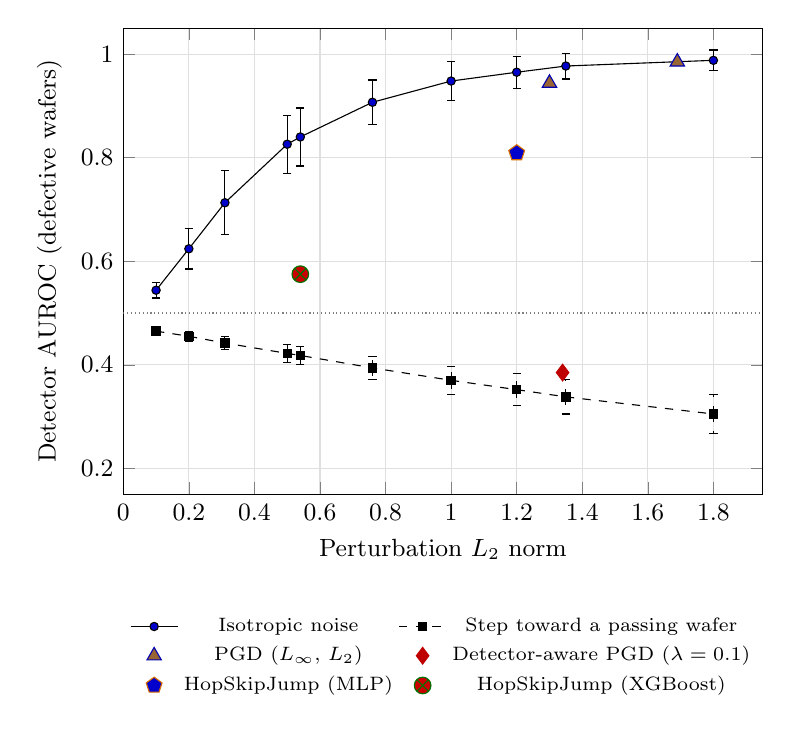
\begin{tikzpicture}
\begin{axis}[width=0.8\textwidth, height=7.5cm, xlabel={Perturbation $L_2$ norm}, ylabel={Detector AUROC (defective wafers)},
  xmin=0, xmax=1.95, ymin=0.15, ymax=1.05, grid=major, grid style={gray!25},
  legend style={font=\scriptsize, at={(0.5,-0.24)}, anchor=north, legend columns=2, draw=none}, label style={font=\small}, tick label style={font=\small}]
\addplot+[black, mark=*, mark size=1.5pt, error bars/.cd, y dir=both, y explicit] coordinates {(0.1,0.544) +- (0,0.015) (0.2,0.624) +- (0,0.039) (0.31,0.713) +- (0,0.062) (0.5,0.826) +- (0,0.056) (0.54,0.840) +- (0,0.056) (0.76,0.907) +- (0,0.043) (1.0,0.948) +- (0,0.037) (1.2,0.965) +- (0,0.031) (1.35,0.977) +- (0,0.025) (1.8,0.988) +- (0,0.020)};
\addlegendentry{Isotropic noise}
\addplot+[black, dashed, mark=square*, mark size=1.5pt, mark options={solid}, error bars/.cd, y dir=both, y explicit] coordinates {(0.1,0.465) +- (0,0.006) (0.2,0.455) +- (0,0.010) (0.31,0.442) +- (0,0.012) (0.5,0.422) +- (0,0.017) (0.54,0.418) +- (0,0.018) (0.76,0.394) +- (0,0.022) (1.0,0.370) +- (0,0.027) (1.2,0.352) +- (0,0.031) (1.35,0.338) +- (0,0.033) (1.8,0.305) +- (0,0.038)};
\addlegendentry{Step toward a passing wafer}
\addplot+[only marks, mark=triangle*, mark size=3pt, blue!70!black] coordinates {(1.69,0.985) (1.30,0.944)};
\addlegendentry{PGD ($L_\infty$, $L_2$)}
\addplot+[only marks, mark=diamond*, mark size=3pt, red!75!black] coordinates {(1.34,0.385)};
\addlegendentry{Detector-aware PGD ($\lambda=0.1$)}
\addplot+[only marks, mark=pentagon*, mark size=3pt, orange!85!black] coordinates {(1.20,0.809)};
\addlegendentry{HopSkipJump (MLP)}
\addplot+[only marks, mark=otimes*, mark size=3pt, green!45!black] coordinates {(0.54,0.575)};
\addlegendentry{HopSkipJump (XGBoost)}
\addplot[gray, densely dotted, domain=0:1.95] {0.5};
\end{axis}
\end{tikzpicture}
\caption{Detector AUROC on defective wafers as a function of Euclidean perturbation size for two geometric controls (mean $\pm$ SD over 50 folds), with the evaluated attacks overlaid at their mean $L_2$ norm. At equal size, detection depends on direction.}
\label{fig:sweep}
\end{figure}

\subsection{HopSkipJump}
HopSkipJump was run on 597 defective wafers against the MLP and completed on 519 of 540 against XGBoost. The remaining 21 XGBoost runs exhausted their budget without terminating and are excluded. Because each run starts from an accepted input, every completed run ends with an accepted input, and the informative quantities are the size of the final perturbation and the detector response.

The two targets give different results. Against the MLP the attack converges to a mean $L_2$ norm of 1.20 and is flagged on 58.4\% of wafers, with an AUROC of 0.809 between attacked wafers and their adversarial counterparts. Against XGBoost it converges to a much smaller perturbation ($L_2$ 0.54), is flagged on 25.2\% of wafers, and gives an AUROC of 0.575. The difference follows the Mahalanobis norm of the perturbation, which is 15.1 for the MLP and 3.3 for XGBoost. A decision-based attack is therefore not inherently invisible to the monitor. It evades when the target's decision boundary can be reached with a perturbation of small Mahalanobis norm, which is the case for the tree ensemble and less so for the MLP.

\subsection{Transfer and an Oversampling Artifact}
\label{sec:transfer}
Table~\ref{tab:transfer} reports XGBoost performance on perturbations that were not crafted against it. In the main pipeline, PGD examples from the MLP raise XGBoost FAR from 0.481 to 0.661 and its FRR from 0.252 to 0.516, and examples from the CNN behave similarly. The random sign control leaves FAR unchanged (0.479) and raises FRR only modestly (0.310). Transfer from the neural networks to the tree ensemble is therefore partial and specific to gradient-derived perturbations.

The comparison pipeline gives a very different impression. With Gaussian oversampling applied to unstandardized features, transferred PGD examples produce an XGBoost FAR of 0.054, which could be read as near-complete transfer resistance. The FRR of 0.988 shows what has actually happened, which is that XGBoost rejects almost every perturbed wafer, and random sign perturbations produce the same collapse (FAR 0.010, FRR 0.976). The likely mechanism is a mismatch of scales. On average 15.6 of the 80 selected features have a raw standard deviation below the noise level of 0.05, which means that the synthetic defective rows are spread far outside the range occupied by passing wafers on those features, and the trees learn to treat any departure from that narrow range as a sign of a defect. Clean performance does not reveal the problem (FAR 0.467, FRR 0.243). The detector results are not sensitive to this choice, and detector-aware PGD at $\lambda=0.1$ in the comparison pipeline gives FAR 0.801, a flag rate of 9.3\%, and a joint evasion rate of 0.768.

\begin{table}[!htbp]
\centering
\caption{XGBoost under perturbations not crafted against it, with and without Gaussian oversampling on unstandardized features (mean $\pm$ SD over 50 folds).}
\label{tab:transfer}
\small\setlength{\tabcolsep}{4pt}
\resizebox{0.85\textwidth}{!}{%
\begin{tabular}{lcccc}
\toprule
 & \multicolumn{2}{c}{No oversampling} & \multicolumn{2}{c}{Raw-feature oversamp.} \\
\cmidrule(lr){2-3}\cmidrule(lr){4-5}
Source & FAR & FRR & FAR & FRR \\
\midrule
None (clean) & 0.481 $\pm$ 0.205 & 0.252 $\pm$ 0.139 & 0.467 $\pm$ 0.207 & 0.243 $\pm$ 0.119 \\
MLP PGD $L_\infty$ & 0.661 $\pm$ 0.216 & 0.516 $\pm$ 0.192 & 0.054 $\pm$ 0.081 & 0.988 $\pm$ 0.036 \\
CNN PGD $L_\infty$ & 0.657 $\pm$ 0.217 & 0.497 $\pm$ 0.192 & 0.083 $\pm$ 0.130 & 0.990 $\pm$ 0.031 \\
Random sign & 0.479 $\pm$ 0.215 & 0.310 $\pm$ 0.176 & 0.010 $\pm$ 0.032 & 0.976 $\pm$ 0.062 \\
\bottomrule
\end{tabular}}
\end{table}

\section{Discussion}
\label{sec:discussion}

\subsection{What the Monitor Measures}
The results are consistent with a simple account. The monitor measures how much of an input's displacement from the training mean lies in directions where the training data show little variation. Perturbations that ignore the covariance structure, whether they come from a gradient attack or from a random number generator, deposit energy in those directions and are flagged. Perturbations that respect the covariance structure are not flagged, whether they arise from an attack that optimizes for this property or from one that happens to find a nearby decision boundary. Inequality~(\ref{eq:bound}) makes the relevant quantity explicit, and the Mahalanobis norms in Table~\ref{tab:detection} broadly order the flag rates of the attacks, with one notable exception. HopSkipJump against XGBoost has a smaller Mahalanobis norm than detector-aware PGD and a higher flag rate, which reflects the fact that the detector-aware attack also controls the sign of the change in score and moves inputs toward the mean.

None of these properties refers to whether the classifier's decision changes. This is the sense in which the monitor's score is decoupled from adversarial harm, and it is in line with earlier findings that detectors can be bypassed by attacks that account for them~\citep{carlini2017detect,tramer2020} and that adversarial examples need not leave the data manifold~\citep{stutz2019}. What the present controls add is a demonstration on industrial tabular data that the decoupling runs in both directions, since the monitor also raises alarms on perturbations that are harmless to the classifier.

\subsection{Implications for Fab Deployment}
The monitor remains useful for the purpose distribution monitoring was designed for. Its sensitivity to isotropic noise at small amplitudes suggests that it would respond to sensor faults, calibration drift, and similar departures from the learned correlation structure, and those are legitimate reasons to hold a wafer for review. What the monitor should not be credited with is protection against an adversary who knows that it is present. Under the white-box assumptions used here, such an adversary gets 0.715 of defective wafers past both the classifier and the monitor, compared with 0.393 that already pass on clean data and 0.008 under an attack that ignores the monitor.

The decision-based attack requires approximately 24,438 queries per wafer, which is a footprint that rate limiting or query auditing at the inference interface could plausibly expose, and it is not available at all to an adversary without query access. The detector-aware gradient attack requires knowledge of the classifier and of the monitor's parameters, which is a strong assumption, although the monitor's parameters are simply the mean and covariance of process data that an insider or a compromised gateway might be able to estimate.

\subsection{Baseline Performance and Practical Significance}
The classifiers evaluated here accept between 0.411 and 0.481 of defective wafers before any attack, which reflects the difficulty of SECOM and limits the practical weight of the absolute FAR values. The conclusions about the monitor do not depend on classifier quality, because they concern how the detector score responds to the geometry of a perturbation. Whether a stronger classifier would be harder to attack within a small Mahalanobis norm is a separate question that these data cannot answer.

\subsection{A Caution on Augmentation}
The oversampling result has a practical lesson that is independent of adversarial robustness. Noise-based oversampling applied before standardization produced a model whose clean metrics were unremarkable and whose response to any small dense perturbation was to reject the wafer. In a robustness evaluation this behavior appears as resistance to transferred attacks, and FAR alone would not reveal it. Reporting FRR alongside FAR under perturbation, and including a random perturbation control, were sufficient to expose the artifact.

\subsection{Limitations}
SECOM is a 2008 benchmark with anonymized features, and it is the only dataset studied, which means that the generality of these findings to other fabs and other tabular industrial settings remains to be established. Perturbations are constrained to training-set ranges in standardized space, which does not guarantee that they correspond to physically realizable sensor readings. Each fold contains roughly 21 defective test wafers, which limits the resolution of FAR and of the AUROC computed on defective wafers, and the 50 folds are dependent. Only one detector is evaluated, and it is a single-Gaussian input-space monitor and not the feature-space method of \citet{lee2018mahal} or other common detectors such as nearest-neighbor distance or isolation forests. The detector flags only large scores, and a two-sided rule might catch some detector-aware examples that sit unusually close to the mean, although an adversary could in turn tune $\lambda$ between the values tested here. The $\lambda$ grid is coarse, and the detector-aware attack assumes full knowledge of the monitor. The CNN applies convolution to features whose adjacency has no physical meaning, although its performance did not depend on feature order. Neural network training on a GPU is not bit-reproducible, and repeated runs of the pipeline differed by about 0.01 in clean FAR, which is small relative to the effects reported here. Finally, 21 of 540 HopSkipJump runs against XGBoost did not terminate within budget and were excluded, which could bias the XGBoost results if those wafers differ systematically from the rest.

\section{Conclusion}
We evaluated input-space Mahalanobis monitoring as a safeguard for semiconductor defect classifiers on SECOM, using controls that separate adversarial harm from perturbation geometry. Random perturbations that do not affect the classifier were flagged on 99.7\% of defective wafers, and a detector-aware PGD attack that raised FAR to 0.765 was flagged on 10.3\%, less often than clean defective wafers. At matched Euclidean size, isotropic noise was detected and displacement toward a real passing wafer was not, and the Mahalanobis norm of the perturbation accounted for the differing detectability of HopSkipJump against the MLP and against XGBoost. An apparent resistance of XGBoost to transferred attacks was traced to Gaussian oversampling on unstandardized features and disappeared when the oversampling was removed.

These results support the use of input-space Mahalanobis monitoring as a monitor of off-distribution sensor behavior and argue against relying on it as a defense against adversaries who are aware of it. For evaluations of similar monitors, we recommend including a random perturbation control, an attack that incorporates the monitor, and a joint metric that counts inputs passing both the classifier and the monitor.

\section*{Declaration of competing interest}
The authors declare that they have no known competing financial interests or personal relationships that could have appeared to influence the work reported in this paper.

\section*{Funding}
This research did not receive any specific grant from funding agencies in the public, commercial, or not-for-profit sectors.

\section*{CRediT authorship contribution statement}
\textbf{David McShannon:} Conceptualization, Methodology, Software, Investigation, Writing -- original draft. \textbf{Abhimanyu Kanwar:} Validation, Writing -- review \& editing. \textbf{Nicholas Dietrich:} Validation, Writing -- review \& editing, Supervision.

\section*{Data availability}
The SECOM dataset is publicly available from the UCI Machine Learning Repository. Code will be made available upon request.

\bibliographystyle{model5-names}
\bibliography{refs}

\end{document}
